\section{Introduction}

3D Gaussian Splatting (3DGS) provides an explicit differentiable representation for dense scene rendering and has become a practical substrate for online visual world modeling~\cite{kerbl20233dgaussian}.
Gaussian SLAM systems such as Photo-SLAM, SplaTAM, GS-SLAM, and Gaussian-SLAM combine camera tracking with dense Gaussian reconstruction~\cite{huai2024photoSLAM,keetha2024splatam,yan2023gs,yugay2023gaussianslam}.
Their tracking frontends and persistent maps, however, still depend on a predominantly static world.
When people or objects occupy a large image region, dynamic observations can corrupt camera estimation and produce persistent Gaussian artifacts.

Semantic and geometric exclusion is therefore a natural defense.
Classical dynamic SLAM removes features associated with movable classes~\cite{bescos2018dynaslam,yu2018ds,xiao2019dynamic}, while recent dynamic Gaussian SLAM systems combine semantics, temporal consistency, depth warping, photometric evidence, or uncertainty to suppress unsafe observations~\cite{xu2024dgslam,kong2024dgsslam,liu2025dyphoslam,zhang2026dagsslam}.
This policy is appropriate for static map construction, but it can be too restrictive for tracking.
A semantic mask can cover visible background, object boundaries, temporarily stationary surfaces, or pixels whose image motion is dominated by camera motion.
Removing all such observations can leave the pose estimator poorly constrained exactly when dynamic occlusion is strongest.

The key issue is not only whether an observation is static, but what authority it should receive.
Tracking and mapping have different failure costs and persistence.
A locally consistent observation may be useful for estimating the current camera pose while still being too uncertain to initialize or optimize persistent static structure.
Treating both decisions with one binary mask conflates \emph{tracking utility} with \emph{map eligibility}.

We propose \textbf{GDOR-SLAM}, a dynamic RGB-D Gaussian SLAM system based on Guarded Dynamic Observation Recovery (GDOR).
GDOR evaluates temporal depth consistency, residual optical-flow consistency, and the current tracking-risk state to recover a conservative subset of observations inside excluded dynamic regions.
Recovered observations may replenish features and support the current camera estimate.
They do not modify the conservative mask used for persistent ORB landmarks or Gaussian initialization, update, and densification.
The method therefore separates transient tracking privilege from persistent map privilege.

\begin{figure*}[t]
  \centering
  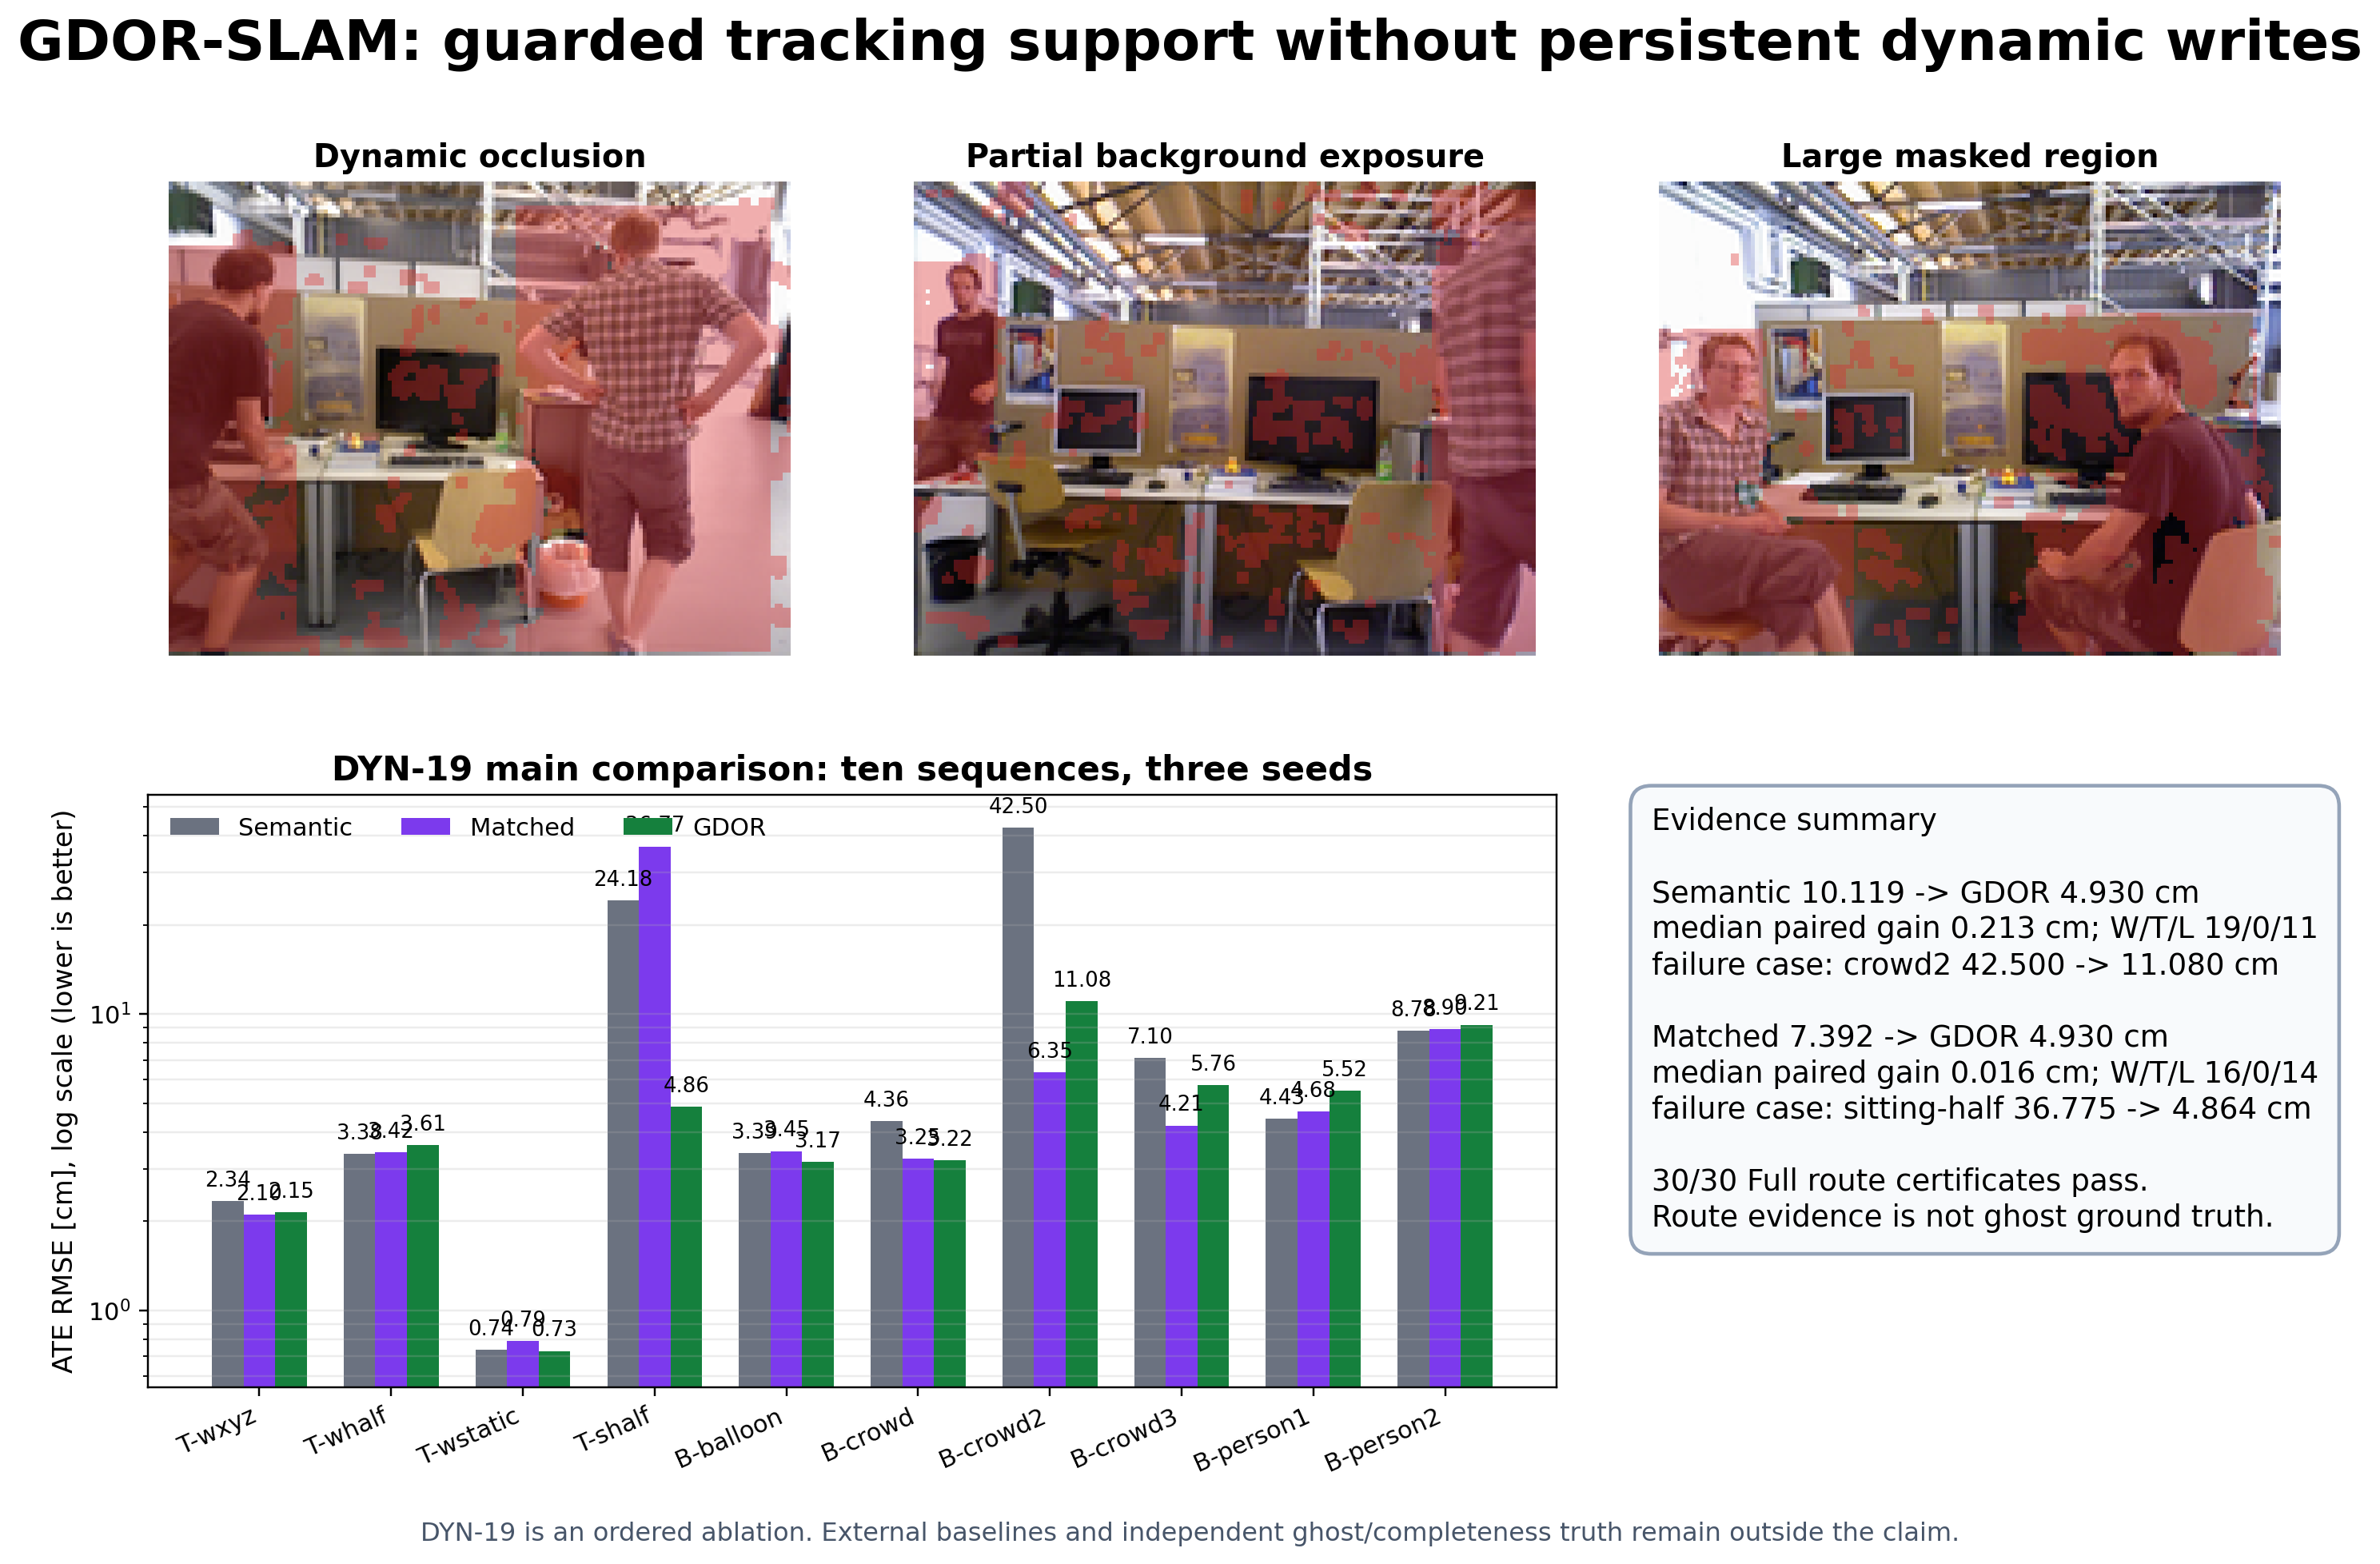
\includegraphics[width=\linewidth]{figures/fig1_overview.png}
  \caption{GDOR-SLAM overview and DYN-19 main evidence. Real TUM dynamic frames show large semantic exclusion regions. The ten-sequence, three-seed comparison exposes both failure-regime rescue and non-uniform cell outcomes against Semantic and the map-matched control. Published external-method values remain context rather than protocol-matched rows.}
  \label{fig:overview}
\end{figure*}

Our contributions are:
\begin{itemize}
    \item We instantiate an auditable two-channel observation contract for RGB-D/ORB Gaussian SLAM: tracking utility does not automatically grant persistent Gaussian map authority.
    \item We introduce GDOR, which combines temporal depth, residual-flow, and tracking-risk evidence to selectively recover dynamic-region observations for transient tracking.
    \item We route the recovered tracking mask and conservative mapping weight independently; the release implements explicit recovered-support overlap, MapPoint-rejection, and RGB-D densification-rejection audits.
    \item We release a completed DYN-19 package with 90 main runs, 120 ordered-ablation runs, 72 multi-seed mapping cells, and per-run route certificates, together with the earlier frozen DYN-15--18 evidence.
\end{itemize}

The supported claim is deliberately bounded.
GDOR improves the DYN-19 aggregate relative to the same-source Semantic and map-matched routes, but the paired results are non-uniform and concentrated in severe failure regimes.
The multi-seed mapping package supplies route and rendering diagnostics, while its occluded-background fields remain proxies rather than independent ghost or completeness truth.
The paper therefore argues for a concrete RGB-D/ORB recovery and routing mechanism rather than conceptual priority, independent component causality, universal improvement, or external SOTA superiority.
